\section{Postgres: Protecting with Azure Backup}
\label{app_pg_s1e2}



\subsection{Restoring from Azure Backup}
The data in our database when performing this test is simply 10000 lines of auto-generated code as shown previously. The result of a "SELECT *"-query is as follows:

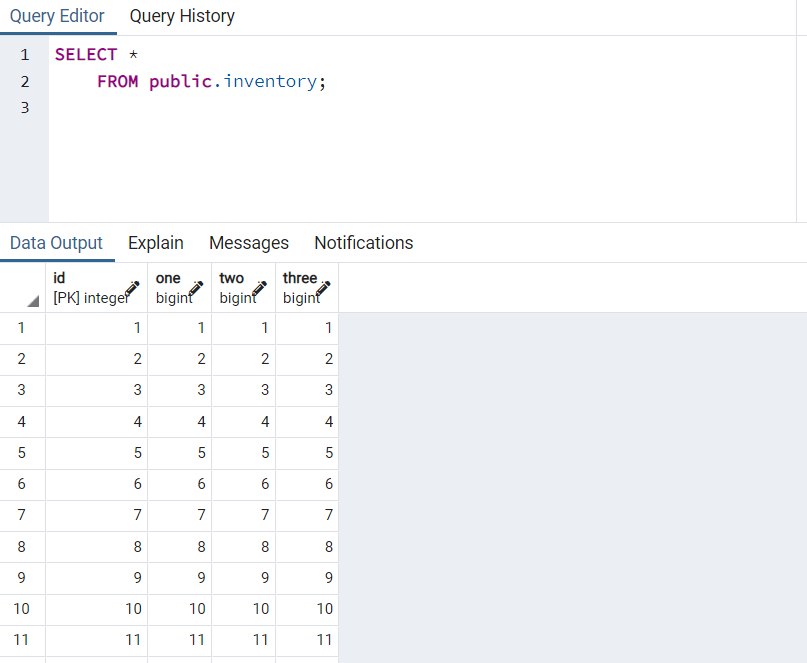
\includegraphics[width=.9\linewidth]{figures/postgresaasmund/12.PNG}

To simulate data loss, we lose some data by dropping table inventory. The same query now returns an error:

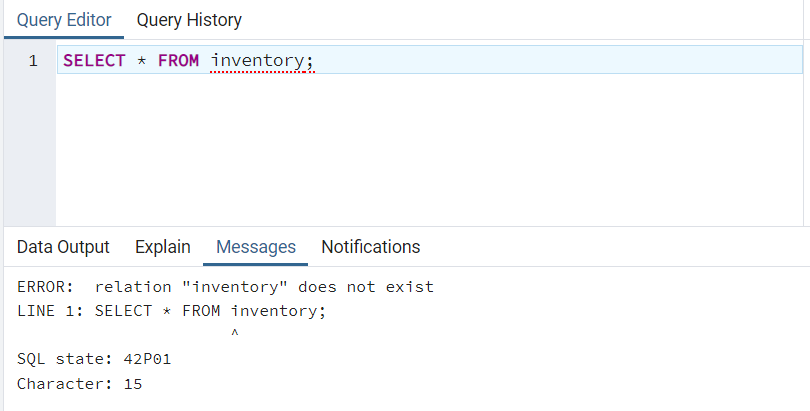
\includegraphics[width=.9\linewidth]{figures/postgresaasmund/10.PNG}

In order to restore from our backup in Azure Backup, we press the "restore"-button on top of the blade. This gives us the following wizard: 

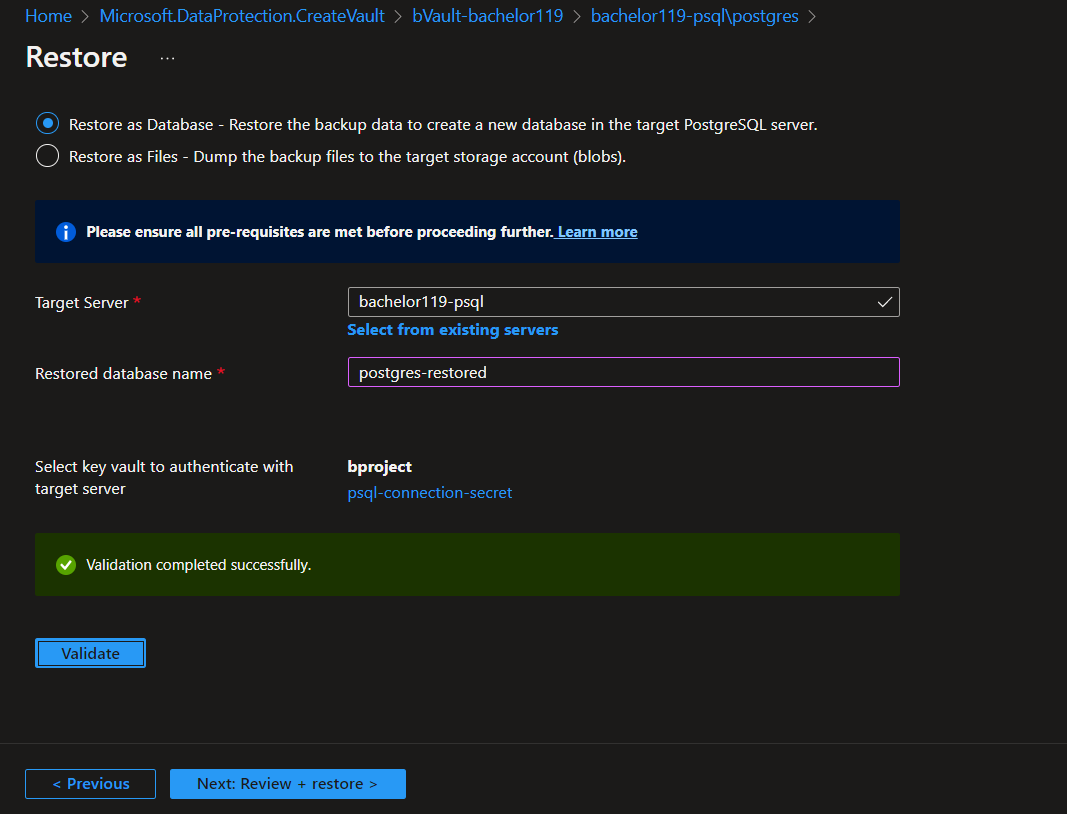
\includegraphics[width=.9\linewidth]{figures/postgresaasmund/11.PNG}

As shown, we are given the option between restoring files or as a database to a server. In this example we choose to restore as a new database on the same server as before. We name this new database "postgres-restored." The same query as before can now be shown on the restored database:

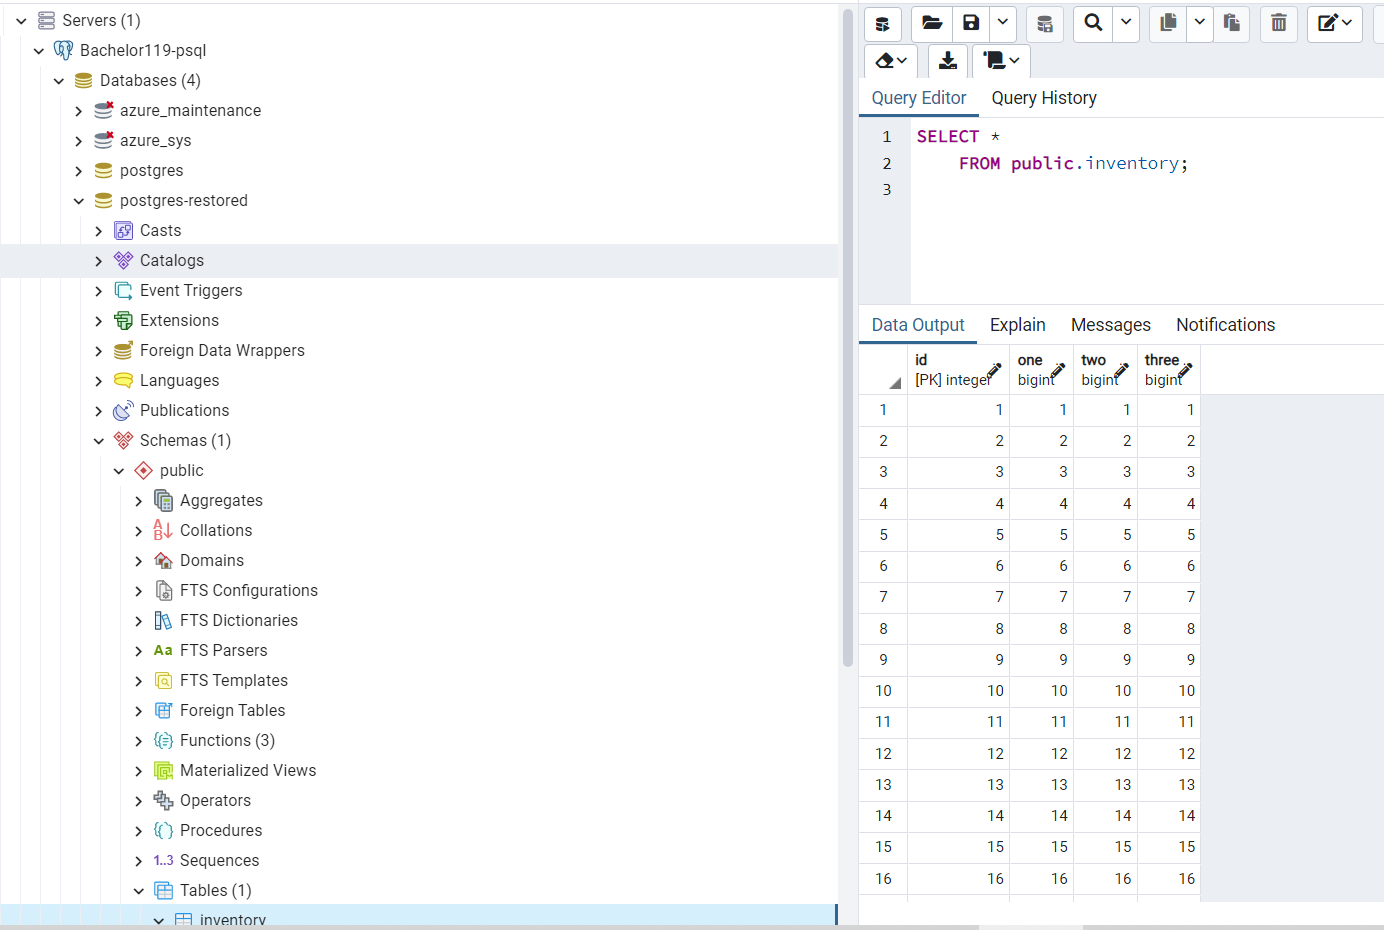
\includegraphics[width=.9\linewidth]{figures/postgresaasmund/13.PNG}

After restoration we can see the successful job in the backup vault:

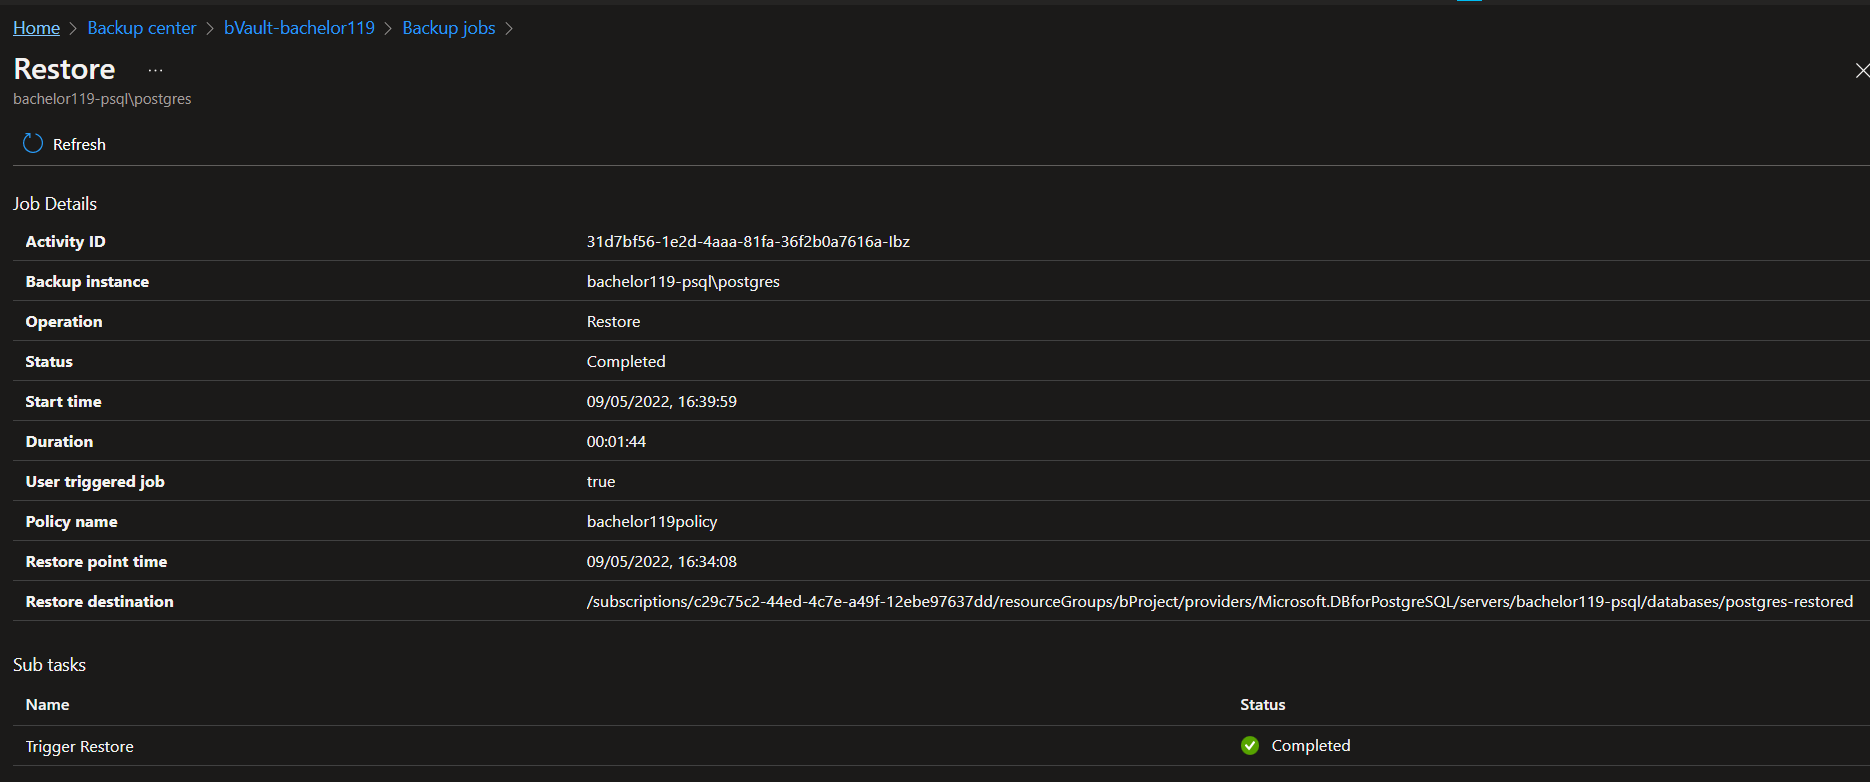
\includegraphics[width=.9\linewidth]{figures/postgresaasmund/14.PNG}




